\documentclass[aspectratio=169,10pt]{beamer}
\usetheme{default}
\usecolortheme{dove}
\setbeamertemplate{navigation symbols}{}
\setbeamertemplate{footline}[frame number]
\usepackage{booktabs}
\usepackage{amsmath}
\usepackage{graphicx}

% numbers and tables written by ../money.py (all macros start with \res)
% written by make_tex.py from money_results.json
\newcommand{\resTau}{20}
\newcommand{\resEps}{0.1}
\newcommand{\resEpsup}{0.49}
\newcommand{\resEpsdown}{0.51}
\newcommand{\resRho}{0.01}
\newcommand{\resBenefit}{2}
\newcommand{\resCost}{1}
\newcommand{\resTol}{10^{-10}}
\newcommand{\resStepsOne}{1}
\newcommand{\resLamOne}{--}
\newcommand{\resLamLinOne}{0.999892}
\newcommand{\resTrelTwo}{15{,}706}
\newcommand{\resHOne}{0.9608}
\newcommand{\resPOne}{0.2402}
\newcommand{\resFitOne}{0.2402}
\newcommand{\resStepsTwoA}{98,106}
\newcommand{\resStepsTwoB}{73,524}
\newcommand{\resTargetOne}{1}
\newcommand{\resTargetTwoA}{249,859}
\newcommand{\resTargetTwoB}{225,283}
\newcommand{\resLamTargetTwoA}{0.999936}
\newcommand{\resLamTargetTwoB}{0.999936}
\newcommand{\resStepsTwo}{249,859}
\newcommand{\resLamTwoA}{0.999936}
\newcommand{\resLamTwoB}{0.999936}
\newcommand{\resLamLinTwoA}{0.999893}
\newcommand{\resLamLinTwoB}{0.907634}
\newcommand{\resFitTwoA}{0.2402}
\newcommand{\resFitTwoB}{0.2345}
\newcommand{\resHelpTwo}{0.9604}
\newcommand{\resWzeroOne}{0.0392}
\newcommand{\resWzeroTwoA}{0.0389}
\newcommand{\resWzeroTwoB}{0.0684}
\newcommand{\resRZero}{0.9608}
\newcommand{\resROne}{0.9608}
\newcommand{\resRTwo}{0.9611}
\newcommand{\resSTwo}{0.1776}
\newcommand{\resGOne}{0.2652}
\newcommand{\resFOne}{0.2760}
\newcommand{\resGTwo}{0.2652}
\newcommand{\resFTwo}{0.2759}
\newcommand{\resGTauTwo}{0.0490}
\newcommand{\resWzeroExactOne}{0.0392}
\newcommand{\resWzeroExactTwoA}{0.0389}
\newcommand{\resWzeroExactTwoB}{0.0684}
\newcommand{\resHTwo}{%
\begin{tabular}{lrr}
\toprule
 & disc & ternary \\
\midrule
disc & $0.9611$ & $0.9316$ \\
ternary & $0.9250$ & $0.8966$ \\
\bottomrule
\end{tabular}}
\newcommand{\resPTwo}{%
\begin{tabular}{lrr}
\toprule
 & disc & ternary \\
\midrule
disc & $0.2403$ & $0.2296$ \\
ternary & $0.2346$ & $0.2242$ \\
\bottomrule
\end{tabular}}


\title{Convergence of score distributions under the money norm}
\date{}

\begin{document}

\begin{frame}{Setup}
  \begin{itemize}
    \item Norm \texttt{CN:000000++ NC:000000--}; noise $\varepsilon=\resEps$, $\varepsilon_\uparrow=\resEpsup$, $\varepsilon_\downarrow=\resEpsdown$.
    \item Strategies: disc \texttt{0,0|g,g}; ternary \texttt{0,0,0|g,g,0|g,g,0} with $\tau=\resTau$.
    \item Payoffs $b=\resBenefit$, $c=\resCost$. Stop when $\mathrm{TV}(w^{t},w^{t-1}) = \tfrac12\sum_j |w^t_j-w^{t-1}_j| \le \resTol$ for every chain.
  \end{itemize}
  \vspace{0.5em}
  \begin{enumerate}
    \item \textbf{Simulation 1.} Disc only, from geometric $\pi_0$ (ratio $\varepsilon_\uparrow/\varepsilon_\downarrow$) $\;\to\;\pi_1$.
    \item \textbf{Simulation 2.} Disc ($1-\rho$) and ternary ($\rho=\resRho$), both from $\pi_1$ $\;\to\;\pi_{2A}$, $\pi_{2B}$.
  \end{enumerate}
  \vspace{0.5em}
  Asymptotic rate: $\mathrm{TV}_t \sim \lambda^t$. For a walk with fixed up rate $g$ and down rate $f>g$,
  $\lambda = 1-(\sqrt f-\sqrt g)^2$.
\end{frame}

\begin{frame}{Stable score distributions}
  \centering
  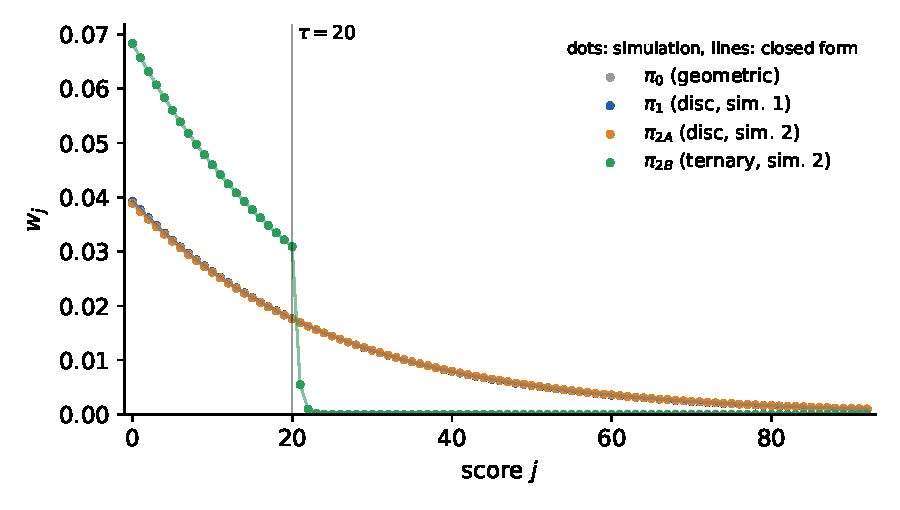
\includegraphics[width=0.78\textwidth]{figures/distributions.pdf}

  \small $w_0$: $\pi_1$ \resWzeroOne, \quad $\pi_{2A}$ \resWzeroTwoA, \quad $\pi_{2B}$ \resWzeroTwoB
\end{frame}

\begin{frame}{Stationary distributions: closed form for every score $j$}
  \small
  Rates (role factor $\lambda=\tfrac14$):\quad
  $g = (1-\varepsilon)\,\lambda\big[(1-w_0^A)(1-\rho)+(1-w_0^B)\rho\big] + \varepsilon\varepsilon_\uparrow$,\quad
  $f = (1-\varepsilon)\,\lambda\big[1-\rho\big(1-\textstyle\sum_{j<\tau}w_j^B\big)\big] + \varepsilon\varepsilon_\downarrow$,\quad
  $g_\tau = \varepsilon\varepsilon_\uparrow$
  \begin{align*}
    \pi_0:\quad    & w_j = (1-r_0)\,r_0^{\,j}, && r_0 = \varepsilon_\uparrow/\varepsilon_\downarrow = \resRZero \\
    \pi_1:\quad    & w_j = (1-r)\,r^{\,j}, && r = g/f = \resGOne/\resFOne = \resROne \quad(\rho=0)\\
    \pi_{2A}:\quad & w_j^A = (1-r)\,r^{\,j}, && r = g/f = \resGTwo/\resFTwo = \resRTwo \\
    \pi_{2B}:\quad & w_j^B =
      \begin{cases}
        w_0^B\, r^{\,j} & j \le \tau \\
        w_0^B\, r^{\,\tau} s^{\,j-\tau} & j > \tau
      \end{cases}
      && s = g_\tau/f = \resGTauTwo/\resFTwo = \resSTwo
  \end{align*}
  \[
    w_0^B = \Big[\tfrac{1-r^{\tau}}{1-r} + \tfrac{r^{\tau}}{1-s}\Big]^{-1}
  \]
  \vspace{-0.5em}
  \begin{center}
    \begin{tabular}{lrr}
      \toprule
      & $w_0$ closed form & $w_0$ simulated \\
      \midrule
      $\pi_1$    & \resWzeroExactOne   & \resWzeroOne \\
      $\pi_{2A}$ & \resWzeroExactTwoA  & \resWzeroTwoA \\
      $\pi_{2B}$ & \resWzeroExactTwoB  & \resWzeroTwoB \\
      \bottomrule
    \end{tabular}
  \end{center}
\end{frame}

\begin{frame}{Time to convergence}
  \begin{columns}[T]
    \begin{column}{0.44\textwidth}
      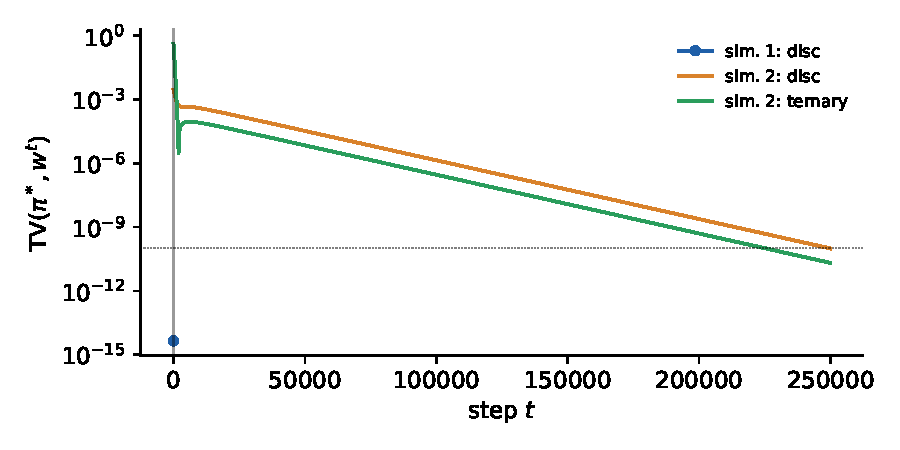
\includegraphics[width=\textwidth]{figures/tv.pdf}
    \end{column}
    \begin{column}{0.55\textwidth}
      \scriptsize
      \setlength{\tabcolsep}{3pt}
      \begin{tabular}{lrrrr}
        \toprule
        & \multicolumn{2}{c}{steps until $\le\resTol$} & & \\
        chain & step TV & $\mathrm{TV}(\pi^*, w^t)$ & $\hat\lambda$ & $\lambda_{\text{lin}}$ \\
        \midrule
        sim.~1 disc    & \resStepsOne  & \resTargetOne  & \resLamOne  & \resLamLinOne \\
        sim.~2 disc    & \resStepsTwoA & \resTargetTwoA & \resLamTwoA & \resLamLinTwoA \\
        sim.~2 ternary & \resStepsTwoB & \resTargetTwoB & \resLamTwoB & \resLamLinTwoB \\
        \bottomrule
      \end{tabular}

      \vspace{0.8em}
      $\pi^*$: closed form. Step TV $\mathrm{TV}(w^t,w^{t-1})$ is still $\le\resTol$ long before
      $w^t$ is that close to $\pi^*$.
      $\hat\lambda$: slope of $\ln\mathrm{TV}_t$ over the second half of the run.
      $\lambda_{\text{lin}}$: closed form with the rates at the top score.
      Sim.~1 starts at its equilibrium ($\pi_0=\pi_1$), so it stops after one step.
      In sim.~2 both chains decay at the same slow rate, set by disc
      (the ternary chain alone would relax at $\lambda_{\text{lin}}$).
      Relaxation time $-1/\ln\hat\lambda \approx \resTrelTwo$ steps.
    \end{column}
  \end{columns}
\end{frame}

\begin{frame}{Helping rates, payoffs and fitness}
  \begin{columns}[T]
    \begin{column}{0.3\textwidth}
      \textbf{Simulation 1} (disc only)
      \vspace{0.5em}

      \begin{tabular}{lr}
        \toprule
        helping rate $H$ & \resHOne \\
        payoff           & \resPOne \\
        fitness          & \resFitOne \\
        \bottomrule
      \end{tabular}
    \end{column}
    \begin{column}{0.68\textwidth}
      \textbf{Simulation 2} ($\rho=\resRho$)
      \vspace{0.5em}

      \small
      $H_{ik}$: Pr(Can of $i$ helps Need of $k$)\\[0.3em]
      \resHTwo

      \vspace{0.6em}
      $P_{ik} = \tfrac14\,(b H_{ki} - c H_{ik})$: payoff to $i$ from meeting $k$\\[0.3em]
      \resPTwo

      \vspace{0.6em}
      Fitness $\sum_k \rho_k P_{ik}$: disc \resFitTwoA, \; ternary \resFitTwoB.
      Population helping rate \resHelpTwo.
    \end{column}
  \end{columns}
\end{frame}

\end{document}
